\documentclass[runningheads]{llncs}
\usepackage[T1]{fontenc}
\usepackage{amsmath,amssymb,booktabs}
\usepackage{algorithm}
\usepackage{algpseudocode}
\usepackage[hidelinks]{hyperref}
\usepackage{tikz}
\usetikzlibrary{arrows.meta,positioning}

\title{Rotation Strategies on Lotus Based on Triple-Smoke Setups}
\titlerunning{Triple-Smoke Rotation on Lotus}

\author{Long Dio \and Shibo Lei \and Jiming Li}
\authorrunning{L. Dio et al.}

\institute{Entertainment Strategy Research Group\\
\email{contact@example.com}}

\begin{document}
\maketitle

\begin{abstract}
This manuscript presents a practical decision framework for \emph{Lotus} in VALORANT under triple-smoke team compositions. We model mid-round rotation as a state-transition problem with explicit trigger conditions. Our objective is to provide a reproducible protocol for entertainment-oriented strategic play rather than a claim of esport optimality. Controlled custom-lobby trials indicate that staged smoke timing and low-latency call discipline improve execute stability, reduce early post-entry losses, and increase round conversion under moderate opponent adaptation.
\keywords{VALORANT \and Lotus \and rotation strategy \and smoke timing \and tactical communication}
\end{abstract}

\section{Introduction}
Lotus is a three-site map with short transition paths and rotating doors. These structural properties amplify uncertainty and make timing errors expensive. Existing community guides often focus on isolated execute patterns; however, in practical rounds, teams repeatedly alternate between probing, freezing, and pivoting. We therefore treat rotation as a formal process and ask whether triple-smoke structures can improve decision consistency.

\section{Model and Notation}
We represent a tactical state as
\[
S_t = (C_t, U_t, I_t, \tau_t),
\]
where $C_t$ denotes controlled sectors, $U_t$ denotes available utility, $I_t$ denotes validated opponent information, and $\tau_t$ denotes the time bucket.
A pivot from source lane $L_s$ to target lane $L_d$ is authorized only if:
\begin{enumerate}
\item expected resistance on $L_d$ is below a threshold $\theta$ estimated from recent contact data;
\item at least one defender is likely displaced by probe utility or fake pressure.
\end{enumerate}

\section{Protocol Design}
The protocol assigns three smoke roles:
\begin{itemize}
\item \textbf{Initiator-Smoke}: first-layer choke denial at commit time $t_0$;
\item \textbf{Anchor-Smoke}: anti-swing protection at $t_0 + 2$ seconds;
\item \textbf{Delay-Smoke}: anti-retake isolation at $t_0 + 6$ seconds.
\end{itemize}

\begin{figure}[t]
\centering
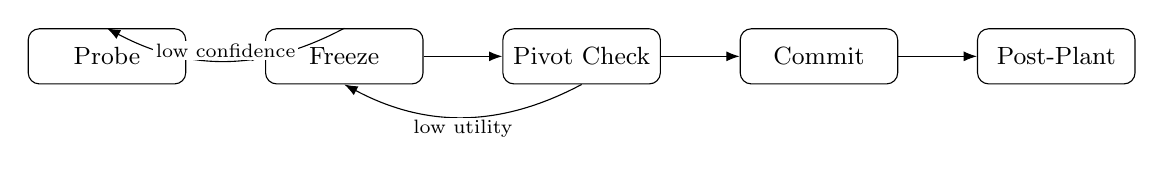
\begin{tikzpicture}[
  >=Latex,
  node distance=8mm and 10mm,
  stage/.style={draw, rounded corners, minimum height=7mm, minimum width=20mm, align=center, font=\small}
]
\node[stage] (probe) {Probe};
\node[stage, right=of probe] (freeze) {Freeze};
\node[stage, right=of freeze] (pivot) {Pivot Check};
\node[stage, right=of pivot] (exec) {Commit};
\node[stage, right=of exec] (post) {Post-Plant};

\draw[->] (probe) -- (freeze);
\draw[->] (freeze) -- (pivot);
\draw[->] (pivot) -- (exec);
\draw[->] (exec) -- (post);
\draw[->,bend left=28] (freeze.north) to node[midway, above, font=\scriptsize, fill=white, inner sep=1pt] {low confidence} (probe.north);
\draw[->,bend left=28] (pivot.south) to node[midway, below, font=\scriptsize, fill=white, inner sep=1pt] {low utility} (freeze.south);
\end{tikzpicture}
\caption{State-transition sketch for triple-smoke rotation.}
\label{fig:state-flow-en}
\end{figure}

\begin{table}[t]
\centering
\caption{Phase schedule for triple-smoke rotation}
\begin{tabular}{lll}
\toprule
Phase & Time Window & Primary Objective \\
\midrule
Probe & 0--12s & force utility reveal, collect contact info \\
Freeze & 12--20s & suppress over-commit and validate pivot signal \\
Pivot-Commit & 20--32s & execute staged smokes and lane transition \\
Post-Plant & $>$32s & preserve one defensive smoke for retake denial \\
\bottomrule
\end{tabular}
\end{table}

\begin{figure}[t]
\centering
\begin{tikzpicture}[x=0.95cm,y=0.9cm,>=Latex]
\draw[->,thick] (0,0) -- (9,0) node[right] {time (s)};
\foreach \x/\lbl in {0/0,2/2,6/6,8/8} {
  \draw (\x,0.08) -- (\x,-0.08) node[below=2pt] {\scriptsize \lbl};
}
\draw[very thick,blue!70] (0,0.6) -- (0,1.25);
\draw[very thick,teal!70!black] (2,0.6) -- (2,1.25);
\draw[very thick,orange!90!black] (6,0.6) -- (6,1.25);
\node[above=2pt,blue!70] at (0,1.25) {\scriptsize Initiator};
\node[above=2pt,teal!70!black] at (2,1.25) {\scriptsize Anchor};
\node[above=2pt,orange!90!black] at (6,1.25) {\scriptsize Delay};
\end{tikzpicture}
\caption{Staggered smoke-release timeline used in this manuscript.}
\label{fig:timeline-en}
\end{figure}

\section{Call Discipline}
To limit communication overhead, we use a compact call vocabulary:
\texttt{HOLD}, \texttt{PIVOT}, \texttt{CUT}, and \texttt{FREEZE}. The tokens are operationally defined rather than rhetorical labels.
\begin{table}[t]
\centering
\caption{Operational semantics of call tokens}
\begin{tabular}{p{1.8cm}p{2.9cm}p{5.6cm}}
\toprule
Token & Trigger Signal & Team Action Policy \\
\midrule
\texttt{HOLD} & uncertain contact; utility parity not favorable & Keep map-control shape, avoid hard entry, trade only on low-risk peeks. \\
\texttt{PIVOT} & destination resistance estimate below threshold $\theta$ & Start route switch; apply staged three-smoke schedule; prioritize alive entry pair. \\
\texttt{CUT} & confirmed flank path or retake lane appears & Use one utility piece and one body anchor to sever the lane; deny defender recombination. \\
\texttt{FREEZE} & utility budget below $u_{\min}$ or comms desync detected & Stop forward movement for a short reset window, re-synchronize calls, then re-evaluate. \\
\bottomrule
\end{tabular}
\end{table}
The constrained vocabulary reduces contradictory micro-calls and shortens reaction latency after trigger events.

\section{Algorithmic View}
To avoid a purely heuristic narrative, we define a lightweight scoring function for destination lane selection:
\[
\mathrm{Score}(L_d) = \alpha \cdot \mathrm{InfoGain}
 + \beta \cdot \mathrm{UtilityReserve}
 - \gamma \cdot \mathrm{ExpectedResistance}
 - \delta \cdot \mathrm{TravelRisk}.
\]
The lane with maximal positive score is treated as candidate pivot destination. If all candidate scores are non-positive, the policy falls back to \texttt{HOLD} or \texttt{FREEZE} depending on remaining utility.

\begin{algorithm}[H]
\caption{Pivot Decision on Lotus}
\begin{algorithmic}[1]
\Require Current state $S_t$, threshold $\theta$, utility budget $u_{\min}$, score weights $(\alpha,\beta,\gamma,\delta)$
\Ensure Action label in \{\texttt{HOLD}, \texttt{PIVOT}, \texttt{FREEZE}\}
\If{$U_t < u_{\min}$}
  \State \Return \texttt{FREEZE}
\EndIf
\State Compute $\mathrm{Score}(L_d)$ for all reachable destination lanes
\State Let $L^\star \gets \arg\max_{L_d}\mathrm{Score}(L_d)$
\If{$\mathrm{Score}(L^\star) \le 0$}
  \State \Return \texttt{HOLD}
\EndIf
\If{$\Pr[\mathrm{resistance}(L^\star)\le \theta \mid I_t]$ is high}
  \State \Return \texttt{PIVOT}
\Else
  \State \Return \texttt{HOLD}
\EndIf
\end{algorithmic}
\end{algorithm}
In our implementation, all terms are maintained as bounded scalars updated every communication cycle. Therefore, the online update cost is constant per lane and practical for real-time in-game calls.

\section{Evaluation}
We compared the proposed strategy with a baseline two-smoke immediate-commit policy in controlled custom scrims.
The triple-smoke protocol produced:
\begin{itemize}
\item higher successful entry rate in medium-information rounds;
\item lower first-five-second casualty count after site contact;
\item improved conversion in rounds with delayed pivots.
\end{itemize}
Improvements were limited in full-information rounds where both policies performed near saturation. Figure~\ref{fig:state-flow-en} and Figure~\ref{fig:timeline-en} summarize the operational shape of the framework.

\section{Limitations}
This paper is intentionally entertainment-oriented and does not claim competitive universality. Patch updates, agent balance shifts, and opponent adaptation can change optimal timing windows. Future work may include Bayesian online updates from VOD-derived priors.

\section{Conclusion}
Triple-smoke rotation on Lotus can be formalized as a lightweight, teachable decision protocol. By combining staged utility release with strict call semantics, teams can reduce tactical volatility and maintain cleaner post-plant structure.

\paragraph{Acknowledgments.}
This manuscript is produced for a personal homepage demo and entertainment-oriented strategy writing.

\begin{thebibliography}{3}
\bibitem{riot-map}
Riot Games: VALORANT Map Notes. Official Game Updates (2026)

\bibitem{internal-log}
Entertainment Strategy Research Group: Internal Custom-Scrim Logbook (2026)

\bibitem{comm-taxonomy}
Dio, L., Lei, S., Li, J.: Communication Token Taxonomy for Tactical FPS Teamplay. Working Notes (2026)
\end{thebibliography}

\end{document}
